\documentclass[10pt,twocolumn]{article}
\usepackage[margin=0.68in,top=0.62in,bottom=0.62in]{geometry}
\usepackage{booktabs}
\usepackage{graphicx}
\usepackage{tikz}
\usetikzlibrary{arrows.meta,positioning}
\usepackage[hidelinks]{hyperref}
\usepackage{caption}
\usepackage{enumitem}
\usepackage{url}
\usepackage{amsmath}
\usepackage{xcolor}
\setlength{\columnsep}{0.22in}
\setlength{\emergencystretch}{2em}
\setlength{\parskip}{3pt}
\setlength{\parindent}{0pt}
\raggedbottom

\title{\vspace{-0.15in}DRC Explain: Verification-Grounded LLM Explanations for SKY130 Layout Checks}
\author{Rana Shamoun and Giovanni Cascone\\
San Jose State University -- CMPE 258 Deep Learning}
\date{December 2026}

\begin{document}
\twocolumn[
\begin{@twocolumnfalse}
\maketitle
\begin{abstract}
We present DRC Explain, a bounded language-model agent for explaining selected SKY130
design-rule checks. The system combines rule retrieval, layout inspection, KLayout
execution, and deterministic verification of structured model claims. It does not
modify layouts or replace physical verification. We evaluate coordinate-only (A),
retrieval-plus-coordinates (B), and tool-grounded (C) conditions across Qwen3 8B,
GPT-4o, and Gemini 3.5 Flash-Lite. GPT-4o and Qwen3 achieve 50/50 C-condition
benchmark verdict accuracy, while Gemini achieves 46/50. The same grids contain
0, 5, and 9 execution errors, respectively. We separately evaluate a 24-layout
held-out set over three repetitions with Qwen3 C, GPT-4o C, and Gemini C. GPT-4o
and Qwen3 remain perfect across repeats; Gemini has substantial provider and
protocol errors. Results are preliminary, are not foundry signoff, and should be
interpreted together with execution reliability.
\end{abstract}
\vspace{0.08in}
\end{@twocolumnfalse}
]

\section{Introduction}
Physical implementation layouts must satisfy manufacturing design rules. KLayout
can identify geometric violations, but engineers often need to determine which rules
apply and explain the evidence in a focused question. A general-purpose language
model may hallucinate thresholds, cite irrelevant rules, or invent scalar
measurements. DRC Explain investigates whether a bounded agent can improve
explanations while geometry remains checked by an established EDA tool.

The project has three objectives:
\begin{enumerate}[leftmargin=*,itemsep=1pt]
\item compare language-only reasoning, rule retrieval, and tool grounding;
\item preserve execution failures as reliability evidence rather than relabeling
      them as geometric results; and
\item evaluate repeated generalization on layouts separated from the development
      benchmark.
\end{enumerate}

The prototype is intentionally narrow. It supports eight curated ordinary
metal1/metal2 width, spacing, and via-enclosure rules on rectangular geometry.
It cannot certify full-chip signoff, wide-metal variants, special regions,
density, antenna, latch-up, routing, or tape-out compliance. PASS and FAIL apply
only to rules selected and checked during the request.

\section{Motivation and Prior Work}
Large language models can generate fluent physical-design explanations, but fluent
text does not establish geometric correctness. Retrieval-augmented generation can
improve access to current documentation, yet retrieved text alone does not verify
actual layout geometry. Tool-using agents address this gap by allowing a model to
request external computations and incorporate tool evidence.

DRC Explain follows a verification-first pattern. The model is responsible for
interpreting the question, selecting supported rules, and producing structured
claims. KLayout remains authoritative for geometry, and a separate verifier
rejects inconsistent claims. The final prose is rendered from verified facts rather
than accepted as unrestricted model output.

This design separates several sources of error: rule-selection errors, geometric
measurement errors, protocol and runtime failures, and overall-verdict errors.
This is especially important because execution failures cannot be inferred from
saved text and must not be converted into PASS or FAIL.

\clearpage
\section{System Architecture}
\begin{center}
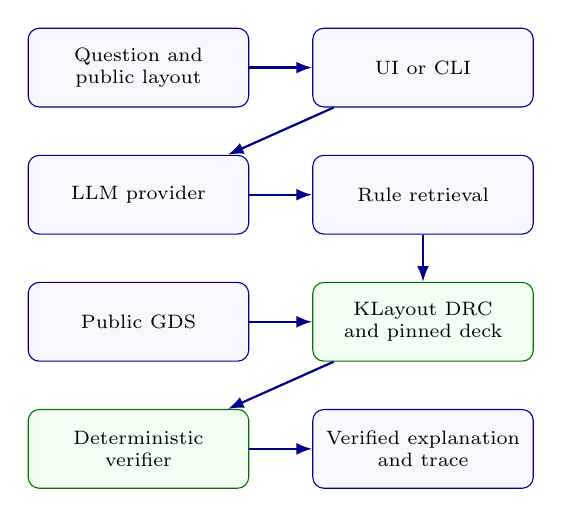
\begin{tikzpicture}[node distance=6mm and 8mm,
 block/.style={draw=blue!55!black,rounded corners,align=center,font=\scriptsize,
 minimum height=10mm,minimum width=28mm,fill=blue!3},
 tool/.style={draw=green!45!black,rounded corners,align=center,font=\scriptsize,
 minimum height=10mm,minimum width=28mm,fill=green!5},
 arrow/.style={-{Latex[length=2mm]},thick,draw=blue!55!black}]
\node[block] (q) {Question and\\public layout};
\node[block,right=of q] (ui) {UI or CLI};
\node[block,below=of q] (llm) {LLM provider};
\node[block,right=of llm] (r) {Rule retrieval};
\node[block,below=of llm] (gds) {Public GDS};
\node[tool,right=of gds] (k) {KLayout DRC\\and pinned deck};
\node[tool,below=of gds] (v) {Deterministic\\verifier};
\node[block,right=of v] (o) {Verified explanation\\and trace};
\draw[arrow] (q)--(ui);
\draw[arrow] (ui)--(llm);
\draw[arrow] (llm)--(r);
\draw[arrow] (r)--(k);
\draw[arrow] (gds)--(k);
\draw[arrow] (k)--(v);
\draw[arrow] (v)--(o);
\end{tikzpicture}
\end{center}
\textit{Fig. 1: The model proposes structured claims; KLayout and the verifier control geometric acceptance.}

The workflow is:
\begin{enumerate}[leftmargin=*,itemsep=1pt]
\item the model receives a public question and layout information;
\item it retrieves only supported rule descriptions and limits;
\item it selects the relevant rule IDs;
\item it requests layout inspection and selected-rule DRC checks;
\item KLayout executes the pinned upstream SKY130 deck;
\item a deterministic verifier compares structured claims with tool evidence;
\item accepted facts are rendered into plain language with source links and traces.
\end{enumerate}

\textbf{Condition A} supplies coordinates only and has no retrieval or DRC tool.
\textbf{Condition B} adds rule retrieval but no geometric tool. \textbf{Condition C}
adds inspection, selected-rule DRC, and deterministic verification.

The agent is read-only. It never writes GDS layouts, moves shapes, routes cells,
or repairs violations. It does not call Magic or OpenROAD. The implementation
therefore demonstrates a tool-using verification agent rather than a layout-editing
or optimization agent.

\clearpage
\section{Tool and Verification Contract}
\subsection{Available tools}
The model-facing tool contract contains three functions:
\begin{itemize}[leftmargin=*,itemsep=1pt]
\item \texttt{retrieve\_rules(query, limit)} searches the curated rule corpus;
\item \texttt{inspect\_layout(gds\_path, top\_cell)} returns layer and rectangle metadata;
\item \texttt{run\_drc(gds\_path, rule\_ids, top\_cell)} runs KLayout and filters evidence
      to requested rules.
\end{itemize}

Although selected-rule filtering is used at the result boundary, the checker executes
the full manufacturing deck. This prevents an expensive or misleading selective DRC
script from becoming the oracle. Public-tool paths are restricted to the public layout
root; evaluator labels and gold reports are inaccessible to the model-facing tools.

\subsection{Structured answer}
The model submits \texttt{selections}, \texttt{claims}, and an overall verdict.
Each claim includes a rule ID, status, limit, available scalar measurements, and
the exact successful DRC call ID. Passing checks have no invented passing distance.
Polygon and corner markers may have no scalar measurement.

\subsection{Verification rules}
The verifier checks:
\begin{enumerate}[leftmargin=*,itemsep=1pt]
\item every selected rule is in the supported retrieved corpus;
\item selections cover every rule that was checked;
\item each claim cites a successful DRC call for the unchanged layout;
\item claimed status and limit match KLayout evidence;
\item available edge-pair measurements match exactly within numerical tolerance;
\item the overall verdict equals FAIL if any selected rule fails, otherwise PASS;
\item REFUSE has no geometric claims and a nonempty reason.
\end{enumerate}

Unrestricted prose is not authoritative. The agent can provide feedback after
rejected claims or prose and continue within a turn budget; other protocol errors
can terminate the run. Invalid or exhausted execution remains ERROR.

\section{Benchmark and Dataset Construction}
The exposed development benchmark has 50 labeled layouts and six unsupported-scope
probes. It includes near-boundary spacing, pass/fail pairs, competing-rule layouts,
and conditional via enclosure. Several layouts and answers were examined during
development; therefore, this benchmark is a sanity check, not an untouched
generalization test.

The oracle for construction comes from a pinned upstream SKY130 KLayout DRC deck.
The project records source revision, deck and layer-map hashes, KLayout versions,
layout hashes, report evidence, and native-RDB cross-checks. This is robust parser
and data validation, but the oracle and implementation share the same KLayout engine.
It is not an independent physical foundry oracle.

\clearpage
\section{Evaluation Methodology}
\subsection{Experimental conditions}
Table~\ref{tab:conditions} summarizes the ablations.
\begin{table}[h]
\centering
\caption{A/B/C experimental conditions.}
\label{tab:conditions}
\small
\begin{tabular}{ll}
\toprule
Condition & Model access \\
\midrule
A & Coordinates only \\
B & Coordinates plus rule retrieval \\
C & Retrieval, inspection, DRC, verification \\
\bottomrule
\end{tabular}
\end{table}

The full grids contain 50 benchmark layouts and six probes per condition. A record
is one model, condition, repetition, and public input. Each frozen model grid contains
168 records. The matching grids use frozen prompt text, implementation hashes, public
input hashes, conditions, and model versions.

\subsection{Fixed-denominator accuracy}
The benchmark verdict accuracy is
\[
\mathrm{Accuracy}_{50}=
\frac{\text{correct accepted benchmark verdicts}}{50}.
\]
Execution ERROR is incorrect in this denominator. REFUSE is also incorrect for a
benchmark layout. This makes the score end-to-end and fixed even when a run fails.

Supplementary metrics include accepted-output count, probe refusal correctness,
rule-selection precision and recall, numeric grounding, pair accuracy, latency,
tool-call count, and provider/runtime metadata. An accepted-output count is never
substituted for fixed-denominator accuracy.

\subsection{Held-out protocol}
A 24-layout held-out set is separate from the original public workflow. It contains
six near-boundary cases, six pass/fail-pair members, six competing-rule layouts,
and six conditional-enclosure layouts. Three unsupported-scope probes are included.
Private labels are kept outside model-facing inputs.

For repeated held-out runs, the denominator is 24 and the mean/range over repetitions
is reported. Original ERROR records are preserved. A retry is placed in a separate
output directory and never selectively replaces a saved failure.

\section{Exposed-Benchmark Results}
\begin{table}[h]
\centering
\caption{Frozen three-model grids, one repetition.}
\label{tab:frozen}
\small
\begin{tabular}{lrrrr}
\toprule
Model & A & B & C & ERROR \\
\midrule
Qwen3 8B & 23/50 & 29/50 & 50/50 & 5 \\
GPT-4o & 29/50 & 27/50 & 50/50 & 0 \\
Gemini & 41/50 & 43/50 & 46/50 & 9 \\
\bottomrule
\end{tabular}
\end{table}

GPT-4o completed all records and all 168 records contained an accepted or ERROR
status. Qwen3 had three B and two C execution errors. Gemini had three A HTTP 503
failures, two B turn-budget failures, and four C protocol failures. Gemini C is
46/50 under the fixed benchmark denominator, not a percentage of only accepted cases.

The frozen grids are controlled for prompt and implementation. However, they are
one-repetition evaluations on a previously exposed benchmark. They support
sanity-check conclusions but not generalization or foundry-signoff claims.

\clearpage
\section{Held-Out Results}
One local Qwen3 8B C run completed all 24 held-out layouts and all three probes.
It achieved 24/24 fixed-denominator benchmark verdict accuracy, 3/3 probe refusals,
and 0 execution ERROR records. Selection recall was 1.000 and numeric grounding was
1.000 for eligible measurements.

The run was repeated three times in a separate directory. Table~\ref{tab:heldout}
shows the repetition-level result.
\begin{table}[h]
\centering
\caption{Qwen3 8B condition C on held-out data.}
\label{tab:heldout}
\small
\begin{tabular}{ccccc}
\toprule
Rep. & Accuracy & Probes & ERROR & Mean s \\
\midrule
1 & 24/24 & 3/3 & 0/27 & 295.6 \\
2 & 24/24 & 3/3 & 0/27 & 279.6 \\
3 & 24/24 & 3/3 & 0/27 & 274.9 \\
\bottomrule
\end{tabular}
\end{table}

Across repetitions, mean held-out accuracy was 100\% and the range was 100--100\%.
Refusal correctness was 1.000, numeric grounding was 1.000, pair accuracy was 1.000,
and no execution ERROR was observed. These values demonstrate repeated stability
for this local model and held-out set, but they do not establish cross-model ranking.

Matching GPT-4o and Gemini 3.5 Flash-Lite held-out C repetitions were completed on
November 25, 2026. Table~\ref{tab:crossheld} summarizes fixed-denominator accuracy.
\begin{table}[h]
\centering
\caption{Held-out condition-C repetitions; Gemini policies are separate runs.}
\label{tab:crossheld}
\small
\begin{tabular}{lcccc}
\toprule
Model & R1 & R2 & R3 & ERROR \\
\midrule
Qwen3 & 24/24 & 24/24 & 24/24 & 0/81 \\
GPT-4o & 24/24 & 24/24 & 24/24 & 0/81 \\
Gemini, original & 20/24 & 14/24 & 15/24 & 23/81 \\
Gemini, 5 retries & 22/24 & 21/24 & 19/24 & 13/81 \\
Gemini, 8 retries & 18/24 & 0/24 & 0/24 & 63/81 \\
\bottomrule
\end{tabular}
\end{table}

The original Gemini run had 22 HTTP 503 errors and one protocol error. With up to
five 503 retries, the separate run had 13 errors; 65 of 78 records encountering
503 completed after retries. Its probe refusals were 1/3, 2/3, and 3/3, not 3/3
throughout. Qwen3, GPT-4o, and the original Gemini run had 3/3 in every repetition.
Provider conditions and implementation differed, so these runs do not establish a
causal improvement from retries.

A subsequent eight-retry run exhausted the free-tier daily request quota: all 63
ERROR records reported HTTP 429. Its probe refusals were 0/3 in every repetition.
These results measure quota-limited execution, not Gemini's answer quality, and are
not pooled with the earlier runs. More retries cannot guarantee availability or
avoid daily quota limits. GPT-4o application-estimate costs were \$0.350, \$0.346,
and \$0.355 per repetition; estimates are not final billing.

The repeated Qwen3 run also exposed a selection-quality limitation. The result audit
recorded six irrelevant citations across conditional-enclosure layouts. These
citations did not change the fixed-denominator overall verdict, but they show that
per-rule selection precision can remain imperfect even when overall verdict accuracy
is perfect.

\section{Failure and Reliability Analysis}
Execution errors are execution failures, not geometric FAIL verdicts and not
domain REFUSes. The primary result preserves this distinction:
\begin{itemize}[leftmargin=*,itemsep=1pt]
\item fixed-denominator accuracy counts every ERROR as incorrect;
\item execution-error rate reports the number of final ERROR records;
\item accepted-output rate reports accepted outputs only;
\item protocol, budget, provider, and tool failures are traceable by type.
\end{itemize}

The held-out Qwen3 run had no ERROR records, whereas the exposed frozen grid had
5 Qwen3 and 9 Gemini errors. This illustrates why execution reliability should be
reported beside answer accuracy. An agent that answers perfectly only on accepted
records is not necessarily reliable end-to-end.

Selection precision and grounding deserve separate presentation. On the held-out
set, overall verdict accuracy was perfect while irrelevant rule selections remained.
This distinction prevents a model that answers the overall question but selects
incorrect surrounding rules from receiving an unqualified completeness claim.

\clearpage
\section{Validity and Limitations}
\begin{itemize}[leftmargin=*,itemsep=2pt]
\item The development and held-out sets are small and curated.
\item The benchmark was exposed during team debugging and demonstrations.
\item The held-out layouts use the same geometry builder and KLayout deck as the
      original benchmark.
\item The oracle and implementation share KLayout, introducing possible shared-tool bias.
\item The project does not evaluate an external OpenROAD or Magic DRC suite.
\item One repetition on each exposed frozen grid provides no run-to-run uncertainty.
\item The three-repetition held-out study covers condition C only; Gemini's later
      retry-policy runs used changed implementations and provider conditions.
\item C verification covers only model-selected rules, not unchecked layout rules.
\item A PASS is not full-chip signoff and is not tape-out certification.
\item Local and hosted hardware, latency, and usage costs are not complete signoff metrics.
\item Human expert layout review has not established physical oracle correctness.
\end{itemize}

These limitations are not merely disclaimers. They determine which claims the project
supports. It supports bounded evidence-grounding and end-to-end execution findings.
It does not support claims of universal DRC expertise, external-suite parity,
general stability across models or workloads, or foundry signoff.

\section{Implementation and Reproducibility}
The repository includes the agent loop, provider adapters, KLayout runner, structured
claim verifier, synthetic benchmark generator, held-out generator and verifier,
experiment runner, local UI, traces, test suite, report drafts, and demo guide.
Saved manifests record provider metadata, prompt and implementation hashes, public
dataset paths, usage, latency, tool calls, verification status, and original errors.
Credentials remain outside source control.

On November 25, 2026, \texttt{run.py check} reported 117 passing automated tests and
one platform-specific skip. The 24 held-out labels passed construction/oracle cross-checking with zero
mismatches and the native-RDB reader cross-check. The first and repeated held-out
runs preserved raw result and trace files under ignored experiment directories.

The implementation demonstrates both software reliability and DRC evidence fidelity,
but raw experiment output is retained separately because model responses and provider
availability can change. A rerun must use a new output directory and declare
repetitions and retry policy before execution.

\clearpage
\section{Discussion}
The exposed results support the interpretation that tool grounding improved
end-to-end result accuracy in the frozen grids. GPT-4o and Qwen3 reached 50/50 C
accuracy, but C combines retrieval, tool access, verification, and rendering.
Therefore, the experiment does not isolate KLayout as a single causal factor.

Gemini led A and B on the exposed benchmark, but its C score and 9 errors show
that a strong coordinate/retrieval prediction does not imply stable tool execution.
This is precisely why fixed-denominator accuracy and accepted-output rates must
be reported together.

The repeated held-out Qwen3 and GPT-4o results provide generalization evidence
within this small test set, yet remain limited. The 24 layouts are separate from
the original examples but are generated and labeled with the same infrastructure.
External-layout or independent-oracle validation would provide stronger evidence.

\section{Future Work}
Additional future work is:
\begin{enumerate}[leftmargin=*,itemsep=1pt]
\item add 24--56 layouts from external open-source or foundry-approved sources;
\item increase support beyond eight rules and rectangular geometry;
\item measure layout-repair or patch generation separately if editing is added;
\item compare KLayout against an independent DRC implementation;
\item estimate confidence intervals or exact binomial intervals for larger held-out sets;
\item add case-level expert review for rule applicability and oracle correctness;
\item record the deterministic 2-minute project demonstration.
\end{enumerate}

If layout repair is introduced, a separate edit loop should propose geometry changes,
write only an isolated output layout, rerun DRC, and verify whether violations were
reduced or new violations were introduced. The current system intentionally does not
perform this additional and potentially unsafe operation.

\clearpage
\section{Conclusion}
DRC Explain combines a language-model agent with a real pinned KLayout DRC workflow
and deterministic claim verification. It does not merely restate rule text; it
retrieves rules, requests geometry evidence, rejects unsupported claims, and renders
explanations from accepted tool facts.

The frozen exposed grids show high C-condition benchmark verdict accuracy but one
repetition and prior development exposure prevent generalization claims. Qwen3 C
and GPT-4o C scored 50/50, and Gemini C scored 46/50, with 5, 0, and 9 execution
errors respectively.

Three held-out Qwen3 C repetitions each achieved 24/24 with 3/3 refusals and no
execution errors. GPT-4o achieved the same outcomes. The original Gemini run scored
20/24, 14/24, and 15/24 with 23 execution errors; a separate five-retry run had
13 errors, and a later eight-retry run encountered daily quota exhaustion.
External-oracle validation remains.

The final report presents both successful measurements and reliability limitations.
The implementation is complete as a bounded verification agent; external validation
and reliable hosted-provider execution remain open work.

\section*{References}
\begin{enumerate}[leftmargin=*,itemsep=1pt]
\item KLayout contributors, \emph{KLayout Documentation and API}, 2026.
\item Efabless and SKY130 PDK contributors, \emph{SkyWater 130 nm PDK}, 2026.
\item OpenAI, \emph{GPT-4o Model Documentation}, 2026.
\item Google, \emph{Gemini API and Function Calling Documentation}, 2026.
\item Alibaba Cloud, \emph{Qwen3 Model Documentation}, 2025.
\item Ollama contributors, \emph{Ollama Local Model Runtime}, 2026.
\item Yao et al., \emph{ReAct: Synergizing Reasoning and Acting in Language Models}, 2023.
\item Lewis et al., \emph{Retrieval-Augmented Generation for Knowledge-Intensive NLP Tasks}, 2020.
\item OpenAI et al., \emph{Tool and Function Calling for Language Models}, 2023--2026.
\item Rana Shamoun and Giovanni Cascone, \emph{DRC Explain Project Repository},
      \url{https://github.com/RanaShamoun/llm-sky130-drc-agent}, 2026.
\end{enumerate}

\end{document}
